% ----------------------------------------------------------------
% AMS-LaTeX Paper ************************************************
% **** -----------------------------------------------------------
%\documentclass{amsart}
%\usepackage{txfonts}
%\documentclass[12pt,oneside]{article}
\documentclass{amsart}
\usepackage{graphicx}
\usepackage{enumitem}
\usepackage{xcolor}
% ----------------------------------------------------------------
\vfuzz2pt % Don't report over-full v-boxes if over-edge is small
\hfuzz2pt % Don't report over-full h-boxes if over-edge is small
% THEOREMS -------------------------------------------------------
\newtheorem{thm}{Theorem}[section]
\newtheorem{cor}[thm]{Corollary}
\newtheorem{lem}[thm]{Lemma}
\newtheorem{prop}[thm]{Proposition}
\theoremstyle{definition}
\newtheorem{defn}[thm]{Definition}
\theoremstyle{Exercise}
\newtheorem{ex}[thm]{Exercise}
\theoremstyle{remark}
\newtheorem{rem}[thm]{Remark}
\theoremstyle{rule}
\newtheorem{rul}[thm]{Rule}

\numberwithin{equation}{section}
% MATH -----------------------------------------------------------
\newcommand{\norm}[1]{\left\Vert#1\right\Vert}
\newcommand{\abs}[1]{\left\vert#1\right\vert}
\newcommand{\set}[1]{\left\{#1\right\}}
\newcommand{\Real}{\mathbb R}
\newcommand{\Z}{\mathbb Z}
\newcommand{\To}{\longrightarrow}
\newcommand{\BX}{\bB(X)}
\newcommand{\A}{\mathcal{A}}
% ----------------------------------------------------------------

% define some simple, commonly-used commands
\newcommand{\eps}{\varepsilon}
\newcommand{\dsum}{\displaystyle\sum}
\newcommand{\dint}{\displaystyle\int}

\newcommand{\pdr}[2]{\dfrac{\partial{#1}}{\partial{#2}}}
\newcommand{\pdrr}[2]{\dfrac{\partial^2{#1}}{\partial{#2}^2}}
\newcommand{\pdrt}[3]{\dfrac{\partial^2{#1}}{\partial{#2}{\partial{#3}}}}
\newcommand{\dr}[2]{\dfrac{d{#1}}{d{#2}}}
\newcommand{\aver}[1]{\langle {#1} \rangle}
\newcommand{\Baver}[1]{\Big\langle {#1} \Big\rangle}

\newcommand{\bzero}{\mathbf 0}
\newcommand{\bGamma}{\mbox{\boldmath{$\Gamma$}}}
\newcommand{\btheta}{\boldsymbol \theta}
\newcommand{\bchi}{\mbox{\boldmath{$\chi$}}}
\newcommand{\bnu}{\boldsymbol \nu}
\newcommand{\bmu}{\boldsymbol \mu}
\newcommand{\brho}{\mbox{\boldmath{$\rho$}}}
\newcommand{\bxi}{\boldsymbol \xi}
\newcommand{\bnabla}{\boldsymbol \nabla}
\newcommand{\bOm}{\boldsymbol \Omega}
\newcommand{\blambda}{\boldsymbol \lambda}
\newcommand{\bsigma}{\boldsymbol \sigma}

\newcommand{\bbR}{\mathbb R}
\newcommand{\bbC}{\mathbb C}
\newcommand{\bbQ}{\mathbb Q}
\newcommand{\bbN}{\mathbb N}
\newcommand{\bbZ}{\mathbb Z}

\newcommand{\ba}{\mathbf a} \newcommand{\bb}{\mathbf b}
\newcommand{\bc}{\mathbf c} \newcommand{\bd}{\mathbf d}
\newcommand{\be}{\mathbf e} \newcommand{\bff}{\mathbf f}
\newcommand{\bg}{\mathbf g} \newcommand{\bh}{\mathbf h}
\newcommand{\bi}{\mathbf i} \newcommand{\bj}{\mathbf j}
\newcommand{\bk}{\mathbf k} \newcommand{\bl}{\mathbf l}
\newcommand{\bm}{\mathbf m} \newcommand{\bn}{\mathbf n}
\newcommand{\bo}{\mathbf o} \newcommand{\bp}{\mathbf p}
\newcommand{\bq}{\mathbf q} \newcommand{\br}{\mathbf r}
\newcommand{\bs}{\mathbf s} \newcommand{\bt}{\mathbf t}
\newcommand{\bu}{\mathbf u} \newcommand{\bv}{\mathbf v}
\newcommand{\bw}{\mathbf w} \newcommand{\bx}{\mathbf x}
\newcommand{\by}{\mathbf y} \newcommand{\bz}{\mathbf z}
\newcommand{\bA}{\mathbf A} \newcommand{\bB}{\mathbf B}
\newcommand{\bC}{\mathbf C} \newcommand{\bD}{\mathbf D}
\newcommand{\bE}{\mathbf E} \newcommand{\bF}{\mathbf F}
\newcommand{\bG}{\mathbf G} \newcommand{\bH}{\mathbf H}
\newcommand{\bI}{\mathbf I} \newcommand{\bJ}{\mathbf J}
\newcommand{\bK}{\mathbf K} \newcommand{\bL}{\mathbf L}
\newcommand{\bM}{\mathbf M} \newcommand{\bN}{\mathbf N}
\newcommand{\bO}{\mathbf O} \newcommand{\bP}{\mathbf P}
\newcommand{\bQ}{\mathbf Q} \newcommand{\bR}{\mathbf R}
\newcommand{\bS}{\mathbf S} \newcommand{\bT}{\mathbf T}
\newcommand{\bU}{\mathbf U} \newcommand{\bV}{\mathbf V}
\newcommand{\bW}{\mathbf W} \newcommand{\bX}{\mathbf X}
\newcommand{\bY}{\mathbf Y} \newcommand{\bZ}{\mathbf Z}

\newcommand{\cA}{\mathcal A} \newcommand{\cB}{\mathcal B}
\newcommand{\cC}{\mathcal C} \newcommand{\cD}{\mathcal D}
\newcommand{\cE}{\mathcal E} \newcommand{\cF}{\mathcal F}
\newcommand{\cG}{\mathcal G} \newcommand{\cH}{\mathcal H}
\newcommand{\cI}{\mathcal I} \newcommand{\cJ}{\mathcal J}
\newcommand{\cK}{\mathcal K} \newcommand{\cL}{\mathcal L}
\newcommand{\cM}{\mathcal M} \newcommand{\cN}{\mathcal N}
\newcommand{\cO}{\mathcal O} \newcommand{\cP}{\mathcal P}
\newcommand{\cQ}{\mathcal Q} \newcommand{\cR}{\mathcal R}
\newcommand{\cS}{\mathcal S} \newcommand{\cT}{\mathcal T}
\newcommand{\cU}{\mathcal U} \newcommand{\cV}{\mathcal V}
\newcommand{\cW}{\mathcal W} \newcommand{\cX}{\mathcal X}
\newcommand{\cY}{\mathcal Y} \newcommand{\cZ}{\mathcal Z}


%%%%%%%%%%%%%%Start%%%%%%%%%%%%%Start%%%%%%%%%%%Start%%%%%%%%%%%%%%%Start%%%%%%%%%%%%%%%%%%%%%%%%%Start%%%%%%%%%%%%%%%%
%%%%%%%%%%%%%%Start%%%%%%%%%%%%%Start%%%%%%%%%%%Start%%%%%%%%%%%%%%%Start%%%%%%%%%%%%%%%%%%%%%%%%%Start%%%%%%%%%%%%%%%%
%%%%%%%%%%%%%%Start%%%%%%%%%%%%%Start%%%%%%%%%%%Start%%%%%%%%%%%%%%%Start%%%%%%%%%%%%%%%%%%%%%%%%%Start%%%%%%%%%%%%%%%%
\usepackage{fancyhdr}

\pagestyle{fancy}
\fancyhf{}
\rhead{}
\chead{\includegraphics[scale=.1]{snhu_logo.png}}

\begin{document}
\begin{center}
\includegraphics[scale=.1]{snhu_logo.png}
\end{center}
\title{\sf Module Six Problem Set}%



\maketitle
This document is proprietary to Southern New Hampshire University. It and the problems within may not be posted on any non-SNHU website.
\\\\\\\\
\begin{center}
%Enter your name below this line:
Ryan Hatch
\end{center}


\begin{center}
\rule{\textwidth}{0.4pt}
\end{center}
\newpage


\section*{}
\section*{}
Directions: Type your solutions into this document and be sure to show all steps for arriving at your solution. Just giving a final number may not receive full credit.
\\

%--------------------------------------------------------------------------------------------------

\section*{Problem 1}


For parts (a) and (b), indicate if each of the two graphs are equal. Justify your answer.\\
 \begin{enumerate}[label=(\alph*)]
 

  \item
   \fbox{
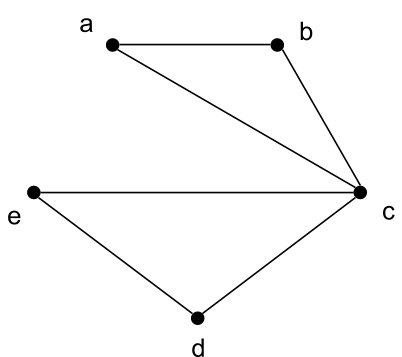
\includegraphics[width=1.5in]{M6-fig1}

}
\hfil
  \fbox{

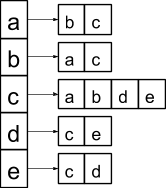
\includegraphics[width=1.5in]{M6-fig2}

}
\\\\
\\\\
 {\color{blue}{\bf Figure 1:} \emph{Left: An undirected graph has 5 vertices. The vertices are arranged in the form of an inverted pentagon. From the top left vertex, moving clockwise, the vertices are labeled: a, b, c, d, and e. Undirected edges, line segments, are between the following vertices: a and b; a and c; b and c; c and d; e and d; and e and c. \\
 }
 }\\
{\color{blue}{\bf Figure 2:} \emph{
  Right: The adjacency list representation of a graph. The list shows all the vertices, a through e, in a column from top to bottom. The adjacent vertices for each vertex in the column are placed in a row to the right of the corresponding vertex’s cell in the column. An arrow points from each cell in the column to its corresponding row on the right. Data from the list, as follows: Vertex a is adjacent to vertices b and c. Vertex b is adjacent to vertices a and c. Vertex c is adjacent to vertices a, b, d, and e. Vertex d is adjacent to vertices c and e. Vertex e is adjacent to vertices c and d.
}
}
\\\\
%Enter your answer below this comment line.
In order to see if the two graphs are equal, I had to make sure that they have the same set of vertices and the same set of edges.\\\\
\textbf{Graph in Figure 1:}\\
Vertices: a, b, c, d, e\\
Edges: ab, ac, bc, cd, ed, ec\\\\
\textbf{Graph (adjacency list) in Figure 2:}\\
Vertex a: connected to b, c\\
Vertex b: connected to a, c\\
Vertex c: connected to a, b, d, e\\
Vertex d: connected to c, e\\
Vertex e: connected to c, d\\\\
The adjacency list for Figure 2 matches the connections in the graph from Figure 1, so these two representations are of the same graph. Thus, the graphs in Figure 1 and Figure 2 are equal.

\newpage
 \item
  \fbox{
   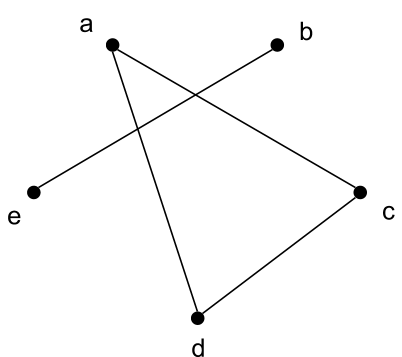
\includegraphics[width=1.5in]{M6-fig3}
}
\hfil
  \fbox{
$
\left( \begin{array}{ccccc}
0 & 0 & 1 & 1 & 0 \\
0 & 0 & 0 & 0 & 1\\
1 & 0 & 0 & 1 & 0\\
1 & 0 & 1 & 0 & 1\\
0 & 1 & 0 & 1 & 0
\end{array} \right)
$
}\\\\
\\
\\
   {\color{blue}{\bf Figure 3:} \emph{An undirected graph has 5 vertices. The vertices are arranged in the form of an inverted pentagon. Moving clockwise from the top left vertex a, the other vertices are, b, c, d, and e. Undirected edges, line segments, are between the following vertices: a and c; a and d; d and c; and e and b. 
  \\\\
}
}
%Enter your answer below this comment line.
 To see if adjacency matrix corresponds to the graph in Figure 3.\\\\
Vertices: a, b, c, d, e\\
Edges: ac, ad, dc, eb\\
Adjacency Matrix:\\
a	b	c	d	e\\
a	0	0	1	1	0\\
b	0	0	0	0	1\\
c	1	0	0	1	0\\
d	1	0	1	0	1\\
e	0	1	0	1	0\\\\
\textbf{The adjacency matrix shows the following connections:}\\
Vertex a is connected to c, d\\
Vertex b is connected to e\\
Vertex c is connected to a, d\\
Vertex d is connected to a, c, e\\
Vertex e is connected to b, d\\\\
These connections match the edges listed in the visual representation of the graph in Figure 3. Thus, the graph and its adjacency matrix representation are equal.

 \newpage

 \
%--------------------------------------------------------------------------------------------------

\item Prove that the two graphs below are isomorphic.\\\\
   \fbox{
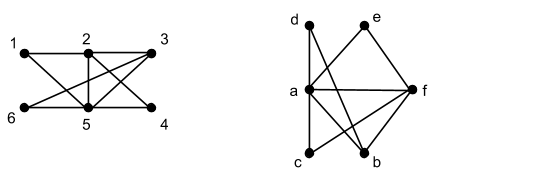
\includegraphics[width=2in]{M6-fig4}
}\\\\
 {\color{blue}{\bf Figure 4:} \emph{Two undirected graphs. Each graph has 6 vertices. The vertices in the first graph are arranged in two rows and 3 columns. From left to right, the vertices in the top row are 1, 2, and 3. From left to right, the vertices in the bottom row are 6, 5, and 4. Undirected edges, line segments, are between the following vertices: 1 and 2; 2 and 3; 1 and 5; 2 and 5; 5 and 3; 2 and 4; 3 and 6; 6 and 5; and 5 and 4. The vertices in the second graph are a through f. Vertices d, a, and c, are vertically inline. Vertices e, f, and b, are horizontally to the right of vertices d, a, and c, respectively. Undirected edges, line segments, are between the following vertices: a and d; a and c; a and e; a and b; d and b; a and f; e and f; c and f; and b and f.
}
}
\\\\
%Enter your answer below this comment line.
For two graphs to be isomorphic, there must be a one-to-one correspondence between their vertices such that the number of edges and the connectivity is preserved.\\\\

\textbf{Graph in the first diagram of Figure 4:}\\
Vertices: 1, 2, 3, 4, 5, 6\\
Edges: 12, 23, 15, 25, 53, 24, 36, 65, 54\\

\textbf{Graph in the second diagram of Figure 4:}\\
Vertices: a, b, c, d, e, f\\
Edges: ad, ac, ae, ab, db, af, ef, cf, bf\\\\
To prove isomorphism, I had to find a mapping from the vertices of the first graph to the second such that the edges correspond.\\\\
For example:\\
Map 1 to a, 2 to d, 3 to c, 4 to f, 5 to e, and 6 to b.\\
If the edges are checked, you will see that each edge in the first graph has a corresponding edge in the second graph with the mapped vertices.\\
Thus, the two graphs are isomorphic because there is a one-to-one correspondence between their vertices that preserves the edges.
\\\\
\item Show that the pair of graphs are not isomorphic by showing that there is a property that is preserved under isomorphism which one graph has and the other does not.\\

\fbox{
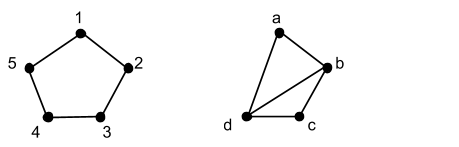
\includegraphics[width=2in]{M6-fig5}
}\\\\
{\color{blue}{\bf Figure 5:} \emph{Two undirected graphs. The first graph has 5 vertices, in the form of a regular pentagon. From the top vertex, moving clockwise, the vertices are labeled: 1, 2, 3, 4, and 5. Undirected edges, line segments, are between the following vertices: 1 and 2; 2 and 3; 3 and 4; 4 and 5; and 5 and 1. The second graph has 4 vertices, a through d. Vertices d and c are horizontally inline, where vertex d is to the left of vertex c. Vertex a is above and between vertices d and c. vertex b is to the right and below vertex a, but above the other two vertices. Undirected edges, line segments, are between the following vertices: a and b; b and c; a and d; d and c; d and b.
}
}
\\
\\
%Enter your answer below this comment line.
To show two graphs are not isomorphic, I had to identify a graph invariant (a property that does not change under isomorphism) that is different in the two graphs.\\\\

In this case, I used the degree sequence as an invariant.\\
The degree sequence for the first graph is (2, 2, 2, 2, 2) since every vertex has exactly two neighbors.\\\\
For the second graph, the degree sequence is (3, 2, 2, 1), since there is one vertex connected to three others, two vertices connected to two others, and one vertex connected to only one other.\\

Since the degree sequences are not the same, the two graphs cannot be isomorphic. Another invariant is the number of cycles: the first graph contains a single cycle that includes all its vertices, whereas the second graph does not have a cycle that includes all its vertices. This also shows that the graphs are not isomorphic.
\\\\

\end{enumerate}    
    
 \newpage

 
%--------------------------------------------------------------------------------------------------

\section*{Problem 2}    
    
Refer to the undirected graph provided below:
\\\\
  \fbox{

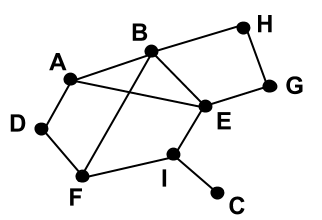
\includegraphics[width=2in]{M6-fig6}

}\\\\
{\color{blue}{\bf Figure 6:} \emph{An undirected graph has 9 vertices. 6 vertices form a hexagon, which is tilted upward to the right. Starting from the leftmost vertex, moving clockwise, the vertices forming the hexagon shape are: D, A, B, E, I, and F. Vertex H is above and to the right of vertex B. Vertex G is the rightmost vertex, below vertex H and above vertex E. Vertex C is the bottom most vertex, a little to the right of vertex E. Undirected edges, line segments, are between the following vertices: A and D; A and B; B and F; B and H; H and G; G and E; B and E; A and E; E and I; I and C; I and F; and F and D.
}
}
\\
\\
    \begin{enumerate}[label=(\roman*)]
        \item What is the maximum length of a path in the graph? Give an example of a path of that length.\\\\
           %Enter your answer here.
           The maximum length of a path is 8. \\
            An example of such a path is C - I - E - G - H - B - A - D - F.
\\\\
        \item What is the maximum length of a cycle in the graph? Give an example of a cycle of that length.\\\\
           %Enter your answer here.
           The maximum length of a cycle is 9.\\
            An example of such a cycle is A - D - F - I - C - I - E - G - H - B - A.
\\\\
        \item Give an example of an open walk of length five in the graph that is a trail but not a path.\\\\
           %Enter your answer here.
           An example of such a trail is D - A - B - H - B - E.
\\\\
        \item Give an example of a closed walk of length four in the graph that is not a circuit.\\\\
           %Enter your answer here.
           An example of this kind of walk is H - B - E - G - H.
\\\\
        \item Give an example of a circuit of length zero in the graph.\\\\
           %Enter your answer here.
           An example of such a circuit is vertex A by itself.
\\\\
    \end{enumerate}
    \newpage
    

%--------------------------------------------------------------------------------------------------

\section*{Problem 3}

\begin{enumerate}[label=(\alph*)]
\item Find the connected components of each graph.\\
    \begin{enumerate}[label=(\roman*)]
    \item $G = (V, \,E).\quad V = \{a,\, b,\, c,\, d,\,  e\}.\quad E = \emptyset$\\\\
%Enter your answer below this comment line.
The connected components are: $\{a\}$, $\{b\}$, $\{c\}$, $\{d\}$, $\{e\}$.
\\\\
    \item $G = (V,\, E).\quad V = \{a,\, b,\, c,\, d,\, e,\, f\}.\quad E = \{ \{c,\, f\}, \,\{a,\, b\},\, \{d,\, a\}, \,\{e,\, c\},\, \{b,\, f\} \}$\\\\
%Enter your answer below this comment line.
The connected component is the entire graph: $\{a, b, c, d, e, f\}$.
\\\\
    \end{enumerate}
\item Determine the edge connectivity and the vertex connectivity of each graph.\\

    \begin{enumerate}[label=(\roman*)]    
 \item
\fbox{

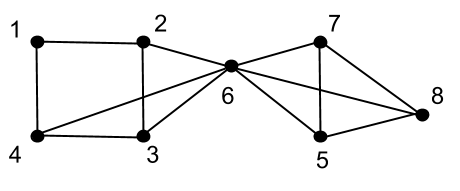
\includegraphics[width=2in]{M6-fig7}

}
\\\\
{\color{blue}{\bf Figure 7:} \emph{An undirected graph has 8 vertices, 1 through 8. 4 vertices form a rectangular-shape on the left. Starting from the top left vertex and moving clockwise, the vertices of the rectangular shape are, 1, 2, 3, and 4. 3 vertices form a triangle on the right, with a vertical side on the left and the other vertex on the extreme right. Starting from the top vertex and moving clockwise, the vertices of the triangular shape are, 7, 8, and 5. Vertex 6 is between the rectangular shape and the triangular shape. Undirected edges, line segments, are between the following vertices: 1 and 2; 2 and 3; 3 and 4; 4 and 1; 2 and 6; 4 and 6; 3 and 6; 6 and 7; 6 and 8; 6 and 5; 7 and 5; 7 and 8; and 5 and 8.
\\
}
}
\\
\\
%Enter your answer below this comment line.
The edge connectivity $\kappa'(G) = 2$ and the vertex connectivity $\kappa(G) = 1$.
\\\\
\newpage
\item  

\fbox{

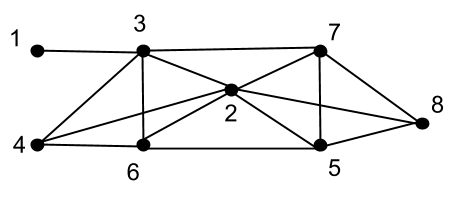
\includegraphics[width=2in]{M6-fig8}

}
\\\\
{\color{blue}{\bf Figure 8:} \emph{An undirected graph has 8 vertices, 1 through 8. 4 vertices form a rectangular shape in the center. Starting from the top left vertex and moving clockwise, the vertices of the rectangular shape are, 3, 7, 5, and 6. Vertex 2 is at about the center of the rectangular shape. Vertex 8 is to the right of the rectangular shape. Vertex 1 and 4 are to the left of the rectangular shape, horizontally in-line with vertices 3 and 6, respectively. Undirected edges, line segments, are between the following vertices: 1 and 3; 3 and 7; 3 and 4; 3 and 6; 3 and 2; 4 and 2; 4 and 6; 6 and 2; 6 and 5; 2 and 5; 2 and 7; 2 and 8; 7 and 5; 7 and 8; and 5 and 8. 
\\
}
}
\\
\\
%Enter your answer below this comment line.
The edge connectivity $\kappa'(G) = 3$ and the vertex connectivity $\kappa(G) = 1$.
\\\\
    \end{enumerate}
\end{enumerate}



 \newpage
%--------------------------------------------------------------------------------------------------

\section*{Problem 4}
For parts (a) and (b) below, find an Euler circuit in the graph or explain why the graph does not have an Euler circuit.\\
\begin{enumerate}[label=(\alph*)]
\item
\fbox{

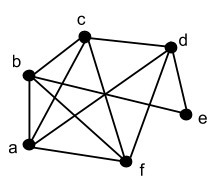
\includegraphics[width=2in]{M6-fig9}\\

}\\\\
{\color{blue}{\bf Figure 9:} \emph{An undirected graph has 6 vertices, a through f. 5 vertices are in the form of a regular pentagon, rotated 90 degrees clockwise. Hence, the top vertex becomes the rightmost vertex. From the bottom left vertex, moving clockwise, the vertices in the pentagon shape are labeled: a, b, c, e, and f. Vertex d is above vertex e, below and to the right of vertex c. Undirected edges, line segments, are between the following vertices: a and b; a and c; a and d; a and f; b and f; b and c; b and e; c and d; d and e; and d and f. Edges c f, a d, and b e intersect at the same point.
\\
}
}
\\
\\
%Enter your answer below this comment line.
There is no Euler circuit in the graph of Figure 9 because all vertices have an odd degree. Therefore, the graph does not have an Euler circuit.
\\\\

\newpage
\item
\fbox{
 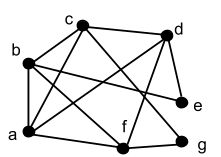
\includegraphics[width=2in]{M6-fig10}
}\\\\
{\color{blue}{\bf Figure 10:} \emph{An undirected graph has 7 vertices, a through g. 5 vertices are in the form of a regular pentagon, rotated 90 degrees clockwise. Hence, the top vertex becomes the rightmost vertex. From the bottom left vertex, moving clockwise, the vertices in the pentagon shape are labeled: a, b, c, e, and f. Vertex d is above vertex e, below and to the right of vertex c. Vertex g is below vertex e, above and to the right of vertex f. Undirected edges, line segments, are between the following vertices: a and b; a and c; a and d; a and f; b and f; b and c; b and e; c and d; c and g; d and e; d and f; and f and g.
\\
}
}
\\
\\
%Enter your answer below this comment line.
The Euler circuit for the graph is `a - b - e - c - d - a - f - g - c - b - f - d - e - g - f - a`.\\
This circuit visits every edge exactly once and returns to the starting vertex, so it is an Euler circuit.
\\\\

\newpage

\item
For each graph below, find an Euler trail in the graph or explain why the graph does not have an Euler trail.\\

{\it (Hint: One way to find an Euler trail is to add an edge between two vertices with odd degree, find an Euler circuit in the resulting graph, and then delete the added edge from the circuit.)}\\
\begin{enumerate}[label=(\roman*)]
\item
\fbox{

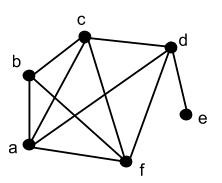
\includegraphics[width=2in]{M6-fig11}\\

}
\\\\
{\color{blue}{\bf Figure 11:} \emph{An undirected graph has 6 vertices, a through f. 5 vertices are in the form of a regular pentagon, rotated 90 degrees clockwise. Hence, the top vertex becomes the rightmost vertex. From the bottom left vertex, moving clockwise, the vertices in the pentagon shape are labeled: a, b, c, e, and f. Vertex d is above vertex e, below and to the right of vertex c. Undirected edges, line segments, are between the following vertices: a and b; a and c; a and d; a and f; b and f; b and c; c and d; c and f; d and e; and d and f.
}
}
\\\\
%Enter your answer below this comment line.
An Euler trail can be created by adding an edge between two vertices with odd degrees and finding an Euler circuit in the modified graph. Then, remove the added edge to have an Euler trail.\\\\
The vertices with odd degrees are a and e. Adding an edge between a and e creates a graph with all even degrees.\\\\
An Euler circuit in the modified graph is `a - b - c - d - e - f - a - d - c - f - b - a`.\\
Removing the added edge between a and e from the circuit results in an Euler trail: `a - b - c - d - e - f - a - d - c - f - b`.
\\\\
\item \fbox{

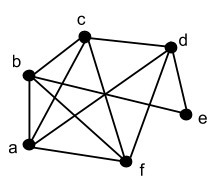
\includegraphics[width=2in]{M6-fig12}\\

}
\\\\
{\color{blue}{\bf Figure 12:} \emph{An undirected graph has 6 vertices, a through f. 5 vertices are in the form of a regular pentagon, rotated 90 degrees clockwise. Hence, the top vertex becomes the rightmost vertex. From the bottom left vertex, moving clockwise, the vertices in the pentagon shape are labeled: a, b, c, e, and f. Vertex d is above vertex e, below and to the right of vertex c. Undirected edges, line segments, are between the following vertices: a and b; a and c; a and d; a and f; b and f; b and c; b and e; c and d; d and e; and d and f. Edges c f, a d, and b e intersect at the same point.
\\
}
}
\\\\
%Enter your answer below this comment line.
The same method used for Figure 11 can also be applied to the graph in Figure 12 to find an Euler trail. The vertices with odd degrees are a and e. Adding an edge between a and e creates a graph with all even degrees.\\
An Euler circuit in the modified graph is `a - b - c - d - e - f - a - d - c - f - b - a`.\\
Removing the added edge between a and e from the circuit results in an Euler trail: `a - b - c - d - e - f - a - d - c - f - b`.

\end{enumerate}
\end{enumerate}
 \newpage
%--------------------------------------------------------------------------------------------------

\section*{Problem 5}

Consider the following tree for a prefix code:\\
\fbox{
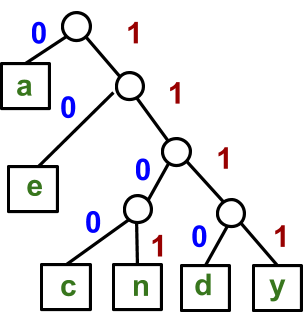
\includegraphics[width=2in]{M6-fig13}\\
}
\\\\
{\color{blue}{\bf Figure 13:} \emph{A tree with 5 vertices. The top vertex branches into character, a, on the left, and a vertex on the right. The vertex in the second level branches into character, e, on the left, and a vertex on the right. The vertex in the third level branches into two vertices. The left vertex in the fourth level branches into character, c, on the left, and character, n, on the right. The right vertex in the fourth level branches into character, d, on the left, and character, y, on the right. The weight of each edge branching left from a vertex is 0. The weight of each edge branching right from a vertex is 1.
\\
}
}
\\
\\

\begin{enumerate}[label=(\alph*)]
\item Use the tree to encode ``day''.\\\\
%Enter your answer below this comment line.
    To encode ``day'' using the tree, I got the following binary sequences for each character:\\
    \begin{itemize}
        \item d: 11\\
        \item a: 0\\
        \item y: 111\\
    \end{itemize}
    Thus, "day" is encoded as 011111.
\\\\
\item Use the tree to encode ``candy''.\\\\
%Enter your answer below this comment line.
    To encode ``candy'' using the tree, I got the following binary sequences for each character:\\
\begin{itemize}
    \item c: 100\\
    \item a: 0\\
    \item n: 101\\
    \item d: 11\\
    \item y: 111\\
\end{itemize}
    Thus, "candy" is encoded as 010010111111.
\\\\
\item Use the tree to decode $``1110101101''$.\\\\
%Enter your answer below this comment line.
    To decode ``1110101101'' using the tree, I followed the binary sequence to get the characters:\\
\begin{itemize}
    \item 111: y\\
    \item 0: a\\
    \item 101: n\\
    \item 10: d\\
\end{itemize}
    The sequence decodes to "yand".
\\\\
\item Use the tree to decode $``111001101110010''$.\\\\
%Enter your answer below this comment line.
    To decode ``111001101110010'' using the tree, I once again followed the binary sequence to get the characters:\\
\begin{itemize}
    \item 111: y\\
    \item 0: a\\
    \item 11: d\\
    \item 0: a\\
    \item 11: d\\
    \item 101: n\\
    \item 0: a\\
    \item 10: d\\
\end{itemize}
    The sequence decodes to "yadadna".
\\\\

\end{enumerate}

 \newpage
%--------------------------------------------------------------------------------------------------

\section*{Problem 6}

\fbox{
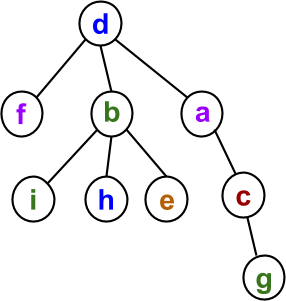
\includegraphics[width=2in]{M6-fig14}\\
}\\\\
{\color{blue}{\bf Figure 14:} \emph{A tree diagram has 9 vertices. The top vertex is d. Vertex d has three branches to vertices, f, b, and a. Vertex b branches to three vertices, i, h, and e. Vertex a branches to vertex c. Vertex c branches to vertex g.
\\
}
}
\\
\\
\begin{enumerate}[label=(\alph*)]
\item Give the order in which the vertices of the tree are visited in a post-order traversal.\\\\
%Enter your answer below this comment line.
    The order in which the vertices of the tree are visited in a post-order traversal is: f, i, h, e, b, g, c, a, d.
\\\\
\item Give the order in which the vertices of the tree are visited in a pre-order traversal.\\\\
%Enter your answer below this comment line.
    The order in which the vertices of the tree are visited in a pre-order traversal is: d, f, b, i, h, e, a, c, g.
\\\\
\end{enumerate}


 \newpage
%--------------------------------------------------------------------------------------------------

\section*{Problem 7}
Consider the following tree. Assume that the neighbors of a vertex are considered in alphabetical order.
\\
\fbox{
 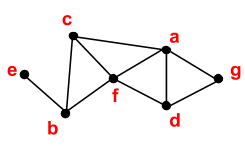
\includegraphics[width=2in]{M6-fig15}\\
}\\\\
{\color{blue}{\bf Figure 15:} \emph{A graph has 7 vertices, a through g, and 10 edges. Vertex e on the left end is horizontally inline with vertex g on the right end. Vertex b is below and to the right of vertex e. Vertex c is above vertex e and to the right of vertex b. Vertex f is between and to the right of vertices c and b. Vertex f is horizontally inline with vertices e and g. Vertex a is above and to the right of vertex f. Vertex d is below and to the right of vertex f. Vertex a is vertically inline with vertex d. Vertex g is between and to the right of vertices a and d. The edges between the vertices are as follows: e and b; b and c; c and f; c and a; a and d; b and f; f and a; f and d; a and g; and d and g.
}
}
\\
\\
\begin{enumerate}[label=(\alph*)]
    \item Give the tree resulting from a traversal of the graph below starting at vertex a using BFS. \\\\
    %Enter your answer below this comment line.
    The tree resulting from a traversal of the graph below starting at vertex a using BFS is:\\
    a -- c -- b -- e, a -- d, a -- f, a -- g.
\\
    \item Give the tree resulting from a traversal of the graph below starting at vertex a using DFS.\\\\
    %Enter your answer below this comment line.
    The tree resulting from a traversal of the graph below starting at vertex a using DFS is:\\
    a -- c -- b -- e, c -- f -- d, a -- g.
\end{enumerate}

\newpage
%--------------------------------------------------------------------------------------------------

\section*{Problem 8}
An undirected weighted graph G is given below:\\\\
\fbox{
 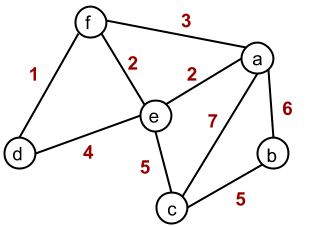
\includegraphics[width=2in]{M6-fig16}\\
}
\\\\
{\color{blue}{\bf Figure 16:} \emph{An undirected weighted graph has 6 vertices, a through f, and 9 edges. Vertex d is on the left. Vertex f is above and to the right of vertex d. Vertex e is below and to the right of vertex f, but above vertex d. Vertex c is below and to the right of vertex e. Vertex a is above vertex e and to the right of vertex c. Vertex b is below and to the right of vertex a, but above vertex c. The edges between the vertices and their weight are as follows: d and f, 1; d and e, 4; f and e, 2; e and a, 2; f and a, 3; e and c, 5; c and a, 7; c and b, 5; and a and b, 6.
\\
}
}
\\
\\
\begin{enumerate}[label=(\alph*)]
\item Use Prim's algorithm to compute the minimum spanning tree for the weighted graph. Start the algorithm at vertex a. Show the order in which the edges are added to the tree.\\\\
%Enter your answer below this comment line.
Using Prim's algorithm starting at vertex a, the minimum spanning tree is constructed by adding the edges in the following order:\\
    \begin{itemize}
        \item Add edge {a, e} with weight 2.\\
        \item Add edge {e, f} with weight 2.\\
        \item Add edge {d, f} with weight 1.\\
        \item Add edge {c, a} with weight 5.\\
        \item Add edge {c, b} with weight 5.\\\\
    \end{itemize}
    The edges added form the minimum spanning tree with a total weight of 15.\\\\

\item What is the minimum weight spanning tree for the weighted graph in the previous question subject to the condition that edge $\{d,\, e\}$ is in the spanning tree?\\\\
    %Enter your answer here.
To include the edge {d, e} in the minimum spanning tree, the edges are added in the following order:\\
    \begin{itemize}
        \item Include edge {d, e} by default.\\
        \item Add edge {d, f} with weight 1.\\
        \item Add edge {e, a} with weight 2.\\
        \item Add edge {e, f} with weight 2.\\
        \item Add edge {c, b} with weight 5.\\\\
    \end{itemize}
The edges added form the minimum spanning tree with the edge {d, e} included and a total weight of 17.\\\\

\item How would you generalize this idea? Suppose you are given a graph G and a particular edge $\{u,\,v\}$ in the graph. How would you alter Prim's algorithm to find the minimum spanning tree subject to the condition that $\{u,\,v\}$ is in the tree?\\\\
%Enter your answer below this comment line.
To generalize this idea for any given edge {u, v} in the graph, Prim's algorithm is modified as follows:\\
\begin{enumerate}
    \item Include the edge {u, v} in the tree from the beginning.\\
    \item Perform Prim's algorithm starting from vertex u or v, considering all other edges except {u, v}.\\
    \item Grow the tree by selecting the edges with the smallest weight while avoiding cycles until all vertices are included in the tree.\\\\
\end{enumerate}
This makes sure that the resulting tree is a minimum spanning tree with the specific edge {u, v} included.
\\\\

\end{document}